\documentclass{article}
\usepackage{amsmath}
\usepackage{amssymb}
\usepackage{tikz}
\usepackage{circuitikz}


\makeatletter
\newcommand*{\encircled}[1]{\relax\ifmmode\mathpalette\@encircled@math{#1}\else\@encircled{#1}\fi}
\newcommand*{\@encircled@math}[2]{\@encircled{$\m@th#1#2$}}
\newcommand*{\@encircled}[1]{%
  \tikz[baseline,anchor=base]{\node[draw,circle,outer sep=0pt,inner sep=.2ex] {#1};}}
\makeatother

\title{AP Physics C: Chapter 23}
\author{Zach Baylin}

\begin{document}
  \maketitle
  \section{Electric Field}
  \begin{itemize}
    \item Positive particle: 
      \begin{tikzpicture}
        \draw (1, 0) node{$\encircled{+}$};
        \draw[->] (.6,0) -- (0,0);
        \draw[->] (1.4,0) -- (2,0);
        \draw[->] (1,.4) -- (1,1);
        \draw[->] (1,-.4) -- (1,-1);
      \end{tikzpicture}
    \item Negative particle:
      \begin{tikzpicture}
        \draw (1, 0) node{$\encircled{-}$};
        \draw[<-] (.6,0) -- (0,0);
        \draw[<-] (1.4,0) -- (2,0);
        \draw[<-] (1,.4) -- (1,1);
        \draw[<-] (1,-.4) -- (1,-1);
      \end{tikzpicture}
    \item Properties of lines:
      \begin{itemize}
        \item continuous curves tangent to field vectors
        \item lines never cross
        \item density of lines represent magnitude
        \item out of $\encircled{+}$ into $\encircled{-}$ or $\infty$
        \item ex.
          \begin{tikzpicture}
            \draw (-2, 0) node{$\encircled{+}$};
            \draw (2, 0)  node{$\encircled{-}$};
            \draw (.2, -.2)  node{$s$};
            \draw[dashed] (0, 1.5) -- (0, -1.5);
            \draw[dashed] (-4, 0) -- (-2.2, 0);
            \draw[dashed] (2.2, 0) -- (4, 0);
            \draw[-] (-1.8, 0) -- (1.8, 0);

            \draw[->, blue] (-0.4, .2) -- (0.4, .2);
            \draw[->, red] (-0.4, .3) -- (0, .3);
            \draw[->, purple] (-0.4, .1) -- (0.8, .1);

            \draw[->, blue] (0, -1) -- (.6, -.8);
            \draw[->, red] (0, -1) -- (.6, -1.2);
            \draw[->, purple] (0, -1) -- (1, -1);
            
            \draw[->, blue] (-3, .2) -- (-3.8, .2);
            \draw[->, red] (-3, .3) -- (-2.6, .3);
            \draw[->, purple] (-3, .1) -- (-3.4, .1);
          \end{tikzpicture}
      \end{itemize}
    \item ex.
      \begin{tikzpicture}
        
      \end{tikzpicture}
    \item \textbf{continuous charge distribution}
      \begin{itemize}
        \item
          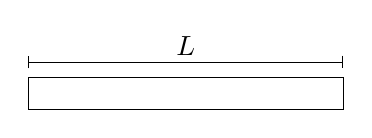
\begin{tikzpicture}
            \draw[|-|] (0, .6) -- (4, .6);
            \draw (2, .8) node{$L$};
            \draw (0,.4) rectangle (4,0);
          \end{tikzpicture}
        \item \underline{uniformly charged}
        \item define $\lambda$ as \textbf{linear charge density}
          \begin{itemize}
            \item $\lambda=\dfrac{Q}{L}$
          \end{itemize}
        \item define $dq=\lambda dL=\dfrac{Q}{L}dL=\dfrac{Q}{L}dx$
        \item $E_{\text{net}}=\sum_i \dfrac{1}{r\pi\varepsilon_0}\cdot\dfrac{dq}{r_i^2}$
      \end{itemize}
  \end{itemize}
\end{document}